Пусть $X_t = y_0 + c \cdot t - \sum\limits_{k=1}^{N_t}\eta_k$, где $\eta_k$ - НОРСВ, неотрицательные и независимые с пуассоновским процессом $N_t$ интенсивности $\lambda$
\\
\\

Величина $X_t$ интерпретируется как капитал страховой компании в момент $t$, $y_0$ - стартовый капитал, $c$ - скорость поступления страховых взносов, $N_t$ - количество страховых исков от начала до момента времени $t$, $\eta_k$ - сумма выплат по $k-$ому страховому случаю
\\
\textbf{Разорение: } $X_t < 0$
\\
\textbf{Момент разорения: } $\tau = inf\{t : X_t < 0\}$
\\
\textbf{Предполагается, что:}
\begin{enumerate}
    \item $\forall v > 0 \ \psi(v) = \mathbb{E}e^{v\eta_t} < \infty$
    \item $\mathbb{E} \eta_1 = a$ и $ c - \lambda a > 0$
\end{enumerate}
\begin{lemma}
Процесс $X_t$ имеет независимые приращения
\end{lemma}
\begin{unnecessary}
\begin{proof}
\\
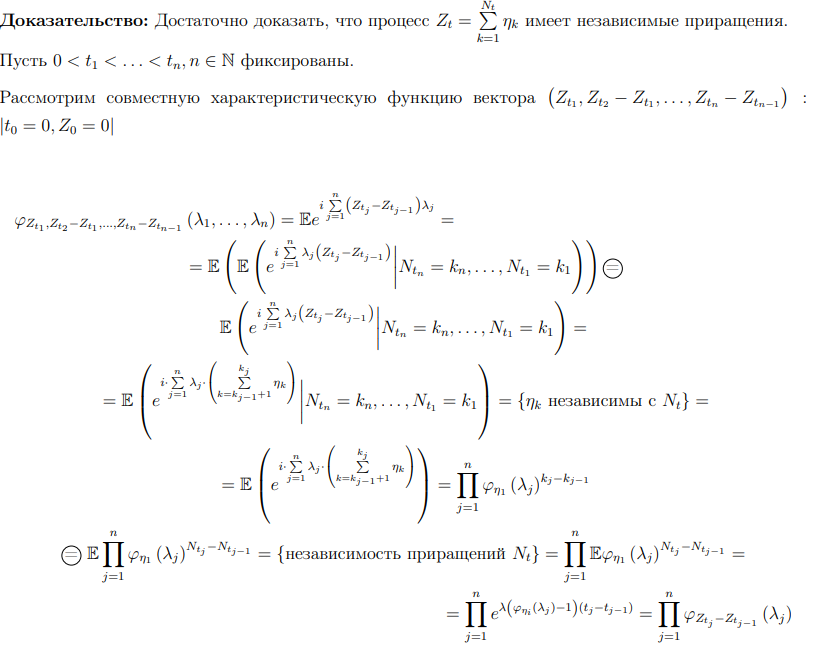
\includegraphics[width=15cm]{images/slup_5.PNG}
\end{proof}
\end{unnecessary}
\begin{lemma}
$\mathbb{E}e^{-v(X_t - X_s)} = e^{(t-s)g(v)}$, где $g(v) = \lambda (\psi(v) - 1) - vc, \ t\geq s, v > 0$
\end{lemma}
\begin{unnecessary}
\begin{proof}
\\
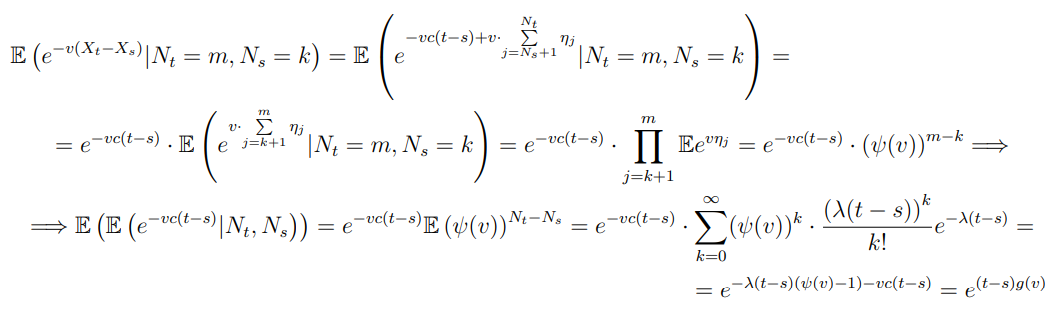
\includegraphics[width=15cm]{images/slup_4.PNG}
\end{proof}
\end{unnecessary}
\begin{lemma}
$Y_t = e^{-vX_t - tg(v)}$ - матрингал относительно $\F^X$
\end{lemma}
\begin{proof}
\\
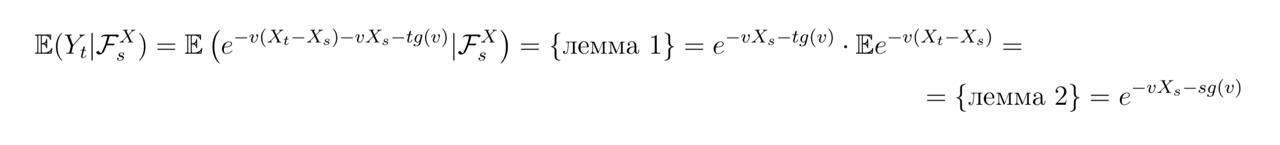
\includegraphics[width=15cm]{images/slup_1.jpg}
\end{proof}
\\
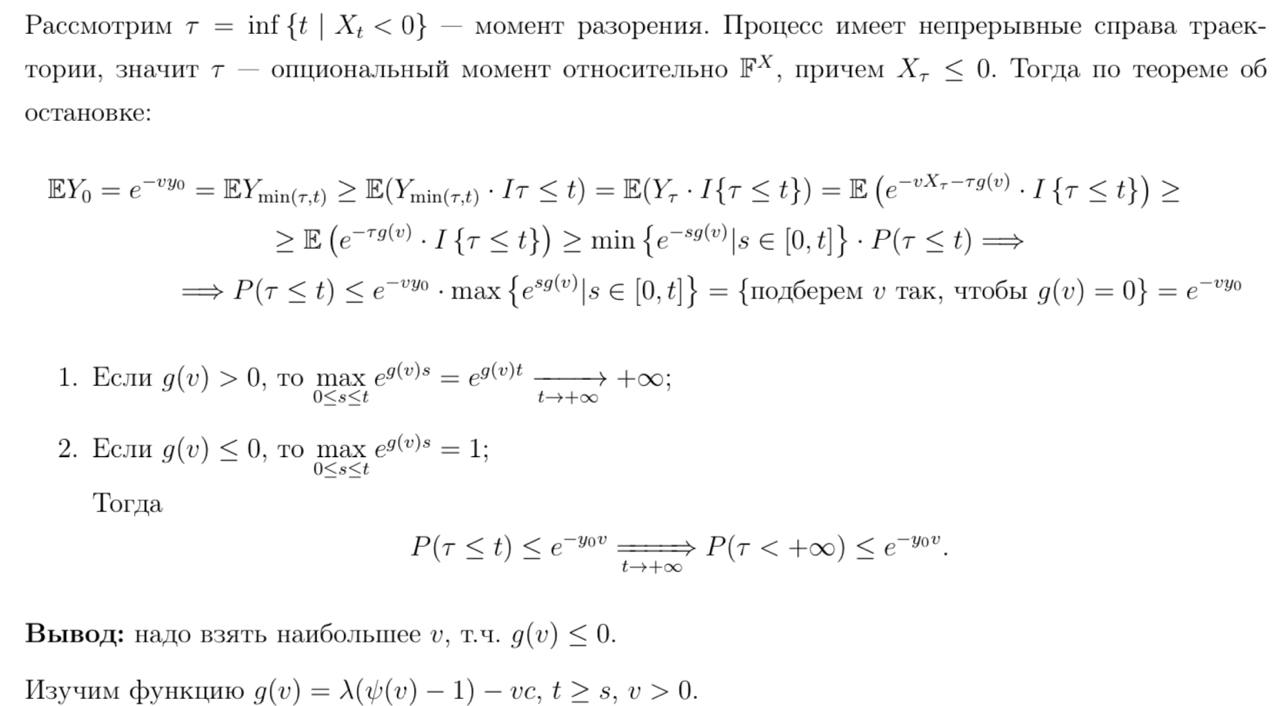
\includegraphics[width=15cm]{images/slup_2.jpg}
\begin{enumerate}
    \item $g(0) = 0$
    \item $g'(v) = \lambda\mathbb{E}(\eta_1e^{v\eta_1} - c$)\\
$g'(0) = \lambda a - c < 0$    
    \item $g''(0) = \lambda \mathbb{E}(\eta_1^2e^{v\eta_1}) > 0$ - возрастающая, тогда $g$ - выпукла вниз
    \item $g(v)$ растет неограниченно
    \\
   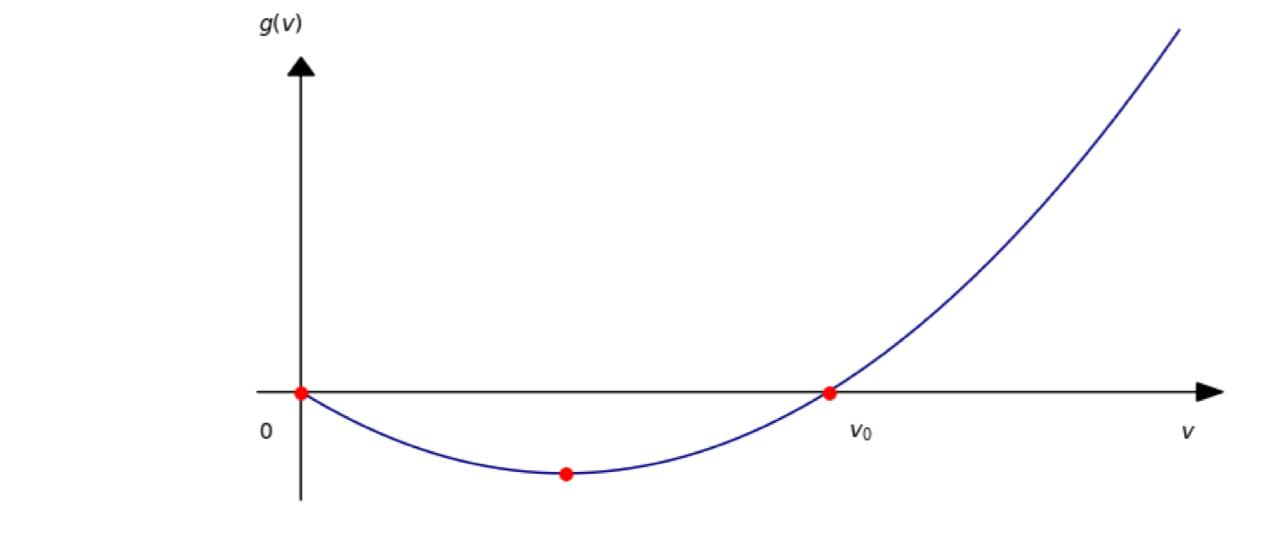
\includegraphics[width=15cm]{images/slup_3.jpg}
\end{enumerate}
\begin{theorem}
Пусть  $ c - \lambda a > 0$,  $\psi(v) = \mathbb{E}e^{v\eta_t}$ конечно $\forall v > 0$, $g(v) = \lambda (\psi(v) - 1) - vc$, $v_0$ - единственный корень уравнения $g(v) = 0$ из $(0, +\infty)$. Тогда
$$P(\tau < + \infty) \leq e^{-y_0v_0}$$
$\tau = inf\{t : X_t < 0\}$
\end{theorem}